\documentclass{article}

\usepackage{arxiv}

\usepackage[utf8]{inputenc}
\usepackage[T1]{fontenc}
\usepackage{hyperref}
\usepackage{url}
\usepackage{booktabs}
\usepackage{amsfonts}
\usepackage{amsmath}
\usepackage{nicefrac}
\usepackage{microtype}
\usepackage{cleveref}
\usepackage{graphicx}
\usepackage{natbib}
\usepackage{doi}
\usepackage{bm}

\graphicspath{{../../assets/figures/}{../../assets/others/}}

\title{Chuck-a-Luck Simulator: A Statistical Inquiry into the Law of Large Numbers and Frequentist Intervals}

\author{
    Axl Roel Andaya, Christian Joseph Bunyi, Sean Higgins Lim \\
    De La Salle University \\
    \texttt{\{axl\_andaya,christian\_bunyi,sean\_higgins\_lim\}} \\ \texttt{@dlsu.edu.ph}
}

% Header overrides
\renewcommand{\shorttitle}{Chuck-a-Luck Statistical Simulator}
\date{}

\begin{document}
\maketitle

% \begin{abstract}
% The abstract.
% \end{abstract}

% \keywords{Chuck-a-Luck \and Law of Large Numbers \and Monte Carlo Simulation \and Frequentist Intervals \and R Shiny \and Maximum Likelihood Estimation}

\section{Introduction}
Chuck-a-Luck, also known as Bird Cage, is a classic dice game that serves as an excellent vehicle for demonstrating fundamental concepts in probability and statistics. This report presents the results of a high-performance simulation engine developed in R Shiny, transitioning the game from a mere gambling activity into a controlled statistical laboratory. Our primary objective is to empirically verify the Law of Large Numbers (LLN) and to evaluate the robustness of various Frequentist Confidence Intervals in quantifying the uncertainty of success probabilities, particularly for rare outcomes.

\section{Theoretical Probability and the House Advantage}
The Chuck-a-Luck gamble is fundamentally a binomial experiment. A player bets on a number $b \in \{1, 2, 3, 4, 5, 6\}$, and three independent fair dice are rolled. The random variable $X$, representing the number of matches, follows a Binomial distribution $B(n=3, p=1/6)$. In this section, we derive the theoretical foundations of the game.

\subsection{Outcome Probability Derivation}
The probability of obtaining exactly $x$ matches is given by the probability mass function (PMF):
\begin{equation}
P(X=x) = \binom{3}{x} \left(\frac{1}{6}\right)^x \left(\frac{5}{6}\right)^{3-x}
\end{equation}

The sample space consists of $6^3 = 216$ equiprobable combinations. Table \ref{tab:outcomes} summarizes the net favorable outcomes and their associated winning probabilities.

\begin{table}[h]
    \centering
    \caption{Chuck-a-Luck Theoretical Outcome Distribution}
    \begin{tabular}{llcc}
        \toprule
        Outcome (Matches) & Combinations & Prob. (Ratio) & Prob. (\%) \\
        \midrule
        0 Matches (Loss) & $1 \times 5 \times 5 \times 5$ & $125/216$ & 57.87\% \\
        1 Match          & $3 \times 1 \times 5 \times 5$ & $75/216$  & 34.72\% \\
        2 Matches         & $3 \times 1 \times 1 \times 5$ & $15/216$  & 6.94\%  \\
        3 Matches         & $1 \times 1 \times 1 \times 1$ & $1/216$   & 0.46\%  \\
        \bottomrule
    \end{tabular}
    \label{tab:outcomes}
\end{table}

\subsection{The House Edge}
The House Edge represents the operator's mathematical advantage. It is calculated as the negative of the Expected Value $E[X]$ for a \$1 wager:
\begin{equation}
E[X] = \sum_{i=0}^{3} P(X=i) \cdot \text{Payout}_i
\end{equation}
Using the standard payout structure ($\{-1, 1, 2, 3\}$), we calculate:
\begin{equation*}
E[X] = \frac{125}{216}(-1) + \frac{75}{216}(1) + \frac{15}{216}(2) + \frac{1}{216}(3) = -\frac{17}{216} \approx -7.87\%
\end{equation*}
This confirms that for every \$100 wagered, a player is statistically expected to lose \$7.87 over the long run.

\section{Computational Framework and Shiny Architecture}
The simulator was developed using the R Shiny framework, optimized for high-throughput Monte Carlo trials.

\subsection{UI Component Design}
\begin{itemize}
    \item \textbf{Sidebar Control Plane:} Allows users to select their target number and simulation parameters, specifically trial count $n$ and payout variations.
    \item \textbf{Dashboard Body:} Features reactive containers including \texttt{valueBox} for real-time metrics and \texttt{plotOutput} for visual analytics.
\end{itemize}

\begin{figure}[h]
    \centering
    %\includegraphics[width=0.8\textwidth]{app_overview.png}
    \caption{The Chuck-a-Luck Simulator dashboard interface showing real-time metrics and initial configuration.}
    \label{fig:app_overview}
\end{figure}

\section{Statistical Methodology and Results}
We utilize the simulation engine to demonstrate frequentist convergence and quantify estimator uncertainty.

\subsection{The Law of Large Numbers (LLN)}
As $n \to \infty$, the MLE estimate $\hat{p} = X/n$ converges to the a priori probability $p=1/6$. The application tracks this convergence sequentially.

\begin{figure}[h]
    \centering
    %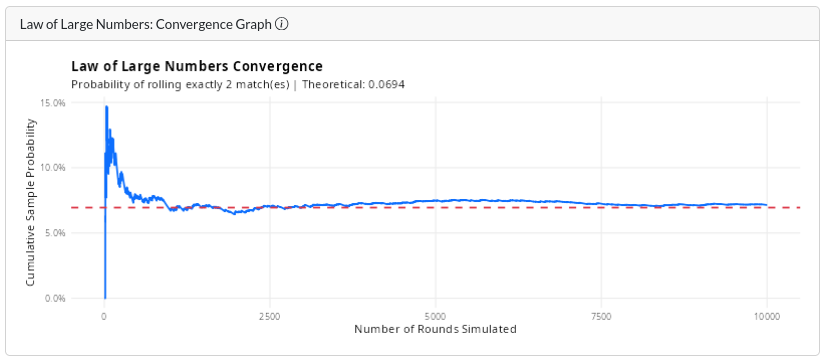
\includegraphics[width=0.8\textwidth]{lln_trace.png}
    \caption{Convergence Trace Plot demonstrating the Law of Large Numbers as the sample proportion stabilizes around the theoretical line.}
    \label{fig:lln}
\end{figure}

\subsection{Frequentist Confidence Intervals}
To quantify uncertainty, we implement three Frequentist intervals. Let $z$ be the $1 - \alpha/2$ quantile of the standard normal distribution:
\begin{itemize}
    \item \textbf{Wald (Standard):} $\hat{p} \pm z \sqrt{\frac{\hat{p}(1-\hat{p})}{n}}$
    \item \textbf{Wilson Score:} $\frac{\hat{p} + \frac{z^2}{2n} \pm z \sqrt{\frac{\hat{p}(1-\hat{p})}{n} + \frac{z^2}{4n^2}}}{1 + \frac{z^2}{n}}$
    \item \textbf{Agresti-Coull:} Improves centering for rare events by adding pseudo-counts.
\end{itemize}

\begin{figure}[h]
    \centering
    %\includegraphics[width=0.8\textwidth]{ci_comparison.png}
    \caption{Comparison of Wald, Wilson, and Agresti-Coull intervals for $X=3$ matches (rare outcome).}
    \label{fig:ci_comparison}
\end{figure}

\begin{figure}[h]
    \centering
    %\includegraphics[width=0.8\textwidth]{ci_behavior.png}
    \caption{Behavior of confidence intervals over increasing trial counts $n$, demonstrating the shrinkage of interval widths.}
    \label{fig:ci_behavior}
\end{figure}

\section{Simulation Performance and AI Integration}
The simulation utilizes a vectorized \texttt{data.table} backend, enabling $n = 10^7$ iterations with sub-second execution.

\subsection{AI Citation}
The development of this project was facilitated by the Antigravity (Gemini) AI assistant. AI was utilized specifically for: (1) multi-file architectural planning, (2) code optimization and vectorization logic in R, and (3) standardization of GitHub-compatible mathematical typesetting across the documentation suite.

\bibliographystyle{unsrtnat}
\bibliography{references}

\end{document}
